%&pdflatex
\documentclass[tikz,border=10pt]{standalone}
\usepackage[utf8]{inputenc}
\usepackage[T2A]{fontenc}

\usepackage{amsmath}
\usepackage{tikz}

\usetikzlibrary{arrows, intersections, calc}

\newcommand{\liq}{\text{L}}
\newcommand{\sol}{\text{S}}

\begin{document}

\footnotesize
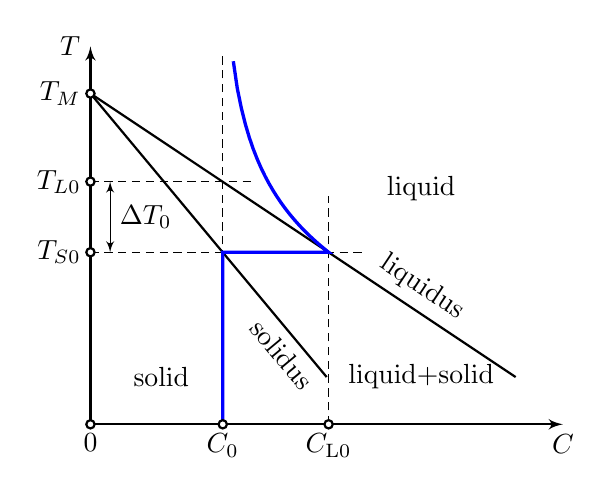
\begin{tikzpicture}[domain=0:4.5,
		solution/.style={blue, very thick},
		boundary/.style={thick},
		mydashed/.style={densely dashed, shorten >=1mm},
		dot/.style = {thick, draw, fill=white, circle, inner sep=0pt, minimum size=3pt},
		>=latex', scale=1.2]

	\path (0,0) coordinate (origin) node[below] {0};
	\path (1.4,0) coordinate (C0) node[below] {$C_0$};
	\path (0,3.5) coordinate (TM) node[left] {$T_M$};

	\node at (0.75,0.5) {solid};
	\node at (3.5,0.5) {liquid+solid};
	\node at (3.5,2.5) {liquid};

	\draw[boundary,->] (origin) -- +(5,0) node[below] {$C$};
	\draw[boundary,->] (origin) -- +(0,4) node[left] {$T$};
	\draw[boundary,name path=liquidus] (TM) -- (4.5,0.5) node[near end, above, sloped] {liquidus};
	\draw[boundary,name path=solidus] (TM) -- (2.5,0.5) node[very near end, below, sloped] {solidus};
	\draw[mydashed,name path=lineC0] (C0) -- +(0,4);

	\path[name intersections={of=solidus and lineC0, by=intS}];
	\path (intS) -- (intS -| TM) coordinate (TS0) node[left] {$T_{S0}$};
	\draw[mydashed,name path=interface] (TS0) -- +(3,0);

	\path[name intersections={of=liquidus and lineC0, by=P}];
	\path (P) -- (P -| TM) coordinate (TL0) node[left] {$T_{L0}$};
	\draw[mydashed] (TL0) -- +(1.8,0);

	\path[name intersections={of=liquidus and interface, by=intL}];
	\path (intL) -- (intL |- C0) coordinate (CL0) node[below] {$C_{\liq0}$};
	\draw[mydashed] (CL0) -- +(0,2.5);

	\begin{scope}[transform canvas={xshift=0.25cm}]
		\draw[<->] (TL0) -- (TS0) node[midway,right] {$\Delta{T}_0$};
	\end{scope}

	\draw[solution] let \p1=($ (CL0)-(C0) $), \n1={veclen(\x1,\y1)*1pt/1cm}
		in (C0) -- (intS) -- (intL) -- plot[shift={(intL)}, domain=0:-\n1*0.9] (\x,{(ln(\n1)-ln(\x+\n1))*25});

	\node[dot] at (origin) {}; \node[dot] at (TM) {};
	\node[dot] at (C0) {}; \node[dot] at (CL0) {};
	\node[dot] at (TS0) {}; \node[dot] at (TL0) {};
\end{tikzpicture}

\end{document}
